\documentclass[a4paper,11pt]{report}
\usepackage[T1]{fontenc}
\usepackage{imakeidx}
\usepackage[pdftex, bookmarks, colorlinks, breaklinks]{hyperref}
\usepackage{graphicx}
\usepackage{caption}
\usepackage{subcaption}
%% TO enhance output
\usepackage{lmodern}
\usepackage{amssymb}

%%Input config
% vim:ft=tex:
%
\usepackage[explicit]{titlesec}
\usepackage{calc} %for \widthof
% Title format: chapter\titleformat{\chapter}[hang]
\titleformat{\chapter}[hang]
{\filcenter}
{\parbox{\widthof{\LARGE\sffamily\MakeUppercase{\chaptername}}}{%
   \filcenter\Large\usefont{T1}{phv}{m}{n}\MakeUppercase{\chaptername}\\%
   \fontsize{48pt}{48pt}\selectfont\thechapter%
 }\enspace%
}
{0pt}
{\Huge\usefont{T1}{phv}{b}{n}\vrule width 1pt \enspace%
 \parbox{\textwidth-\widthof{\LARGE\sffamily\MakeUppercase{\chaptername}\enspace}}{\filright #1}%
}
% Title format: section
%\titleformat{\section}[hang]{\sffamily\bfseries\filright\lsstyle}{}{0em}{\rule[-0.25cm]{1.5pt}{1cm}\quad#1}
\titleformat{\section}[hang]
{\filcenter}
{\parbox{\widthof{\Large\sffamily{Chapter}}}{
        \filcenter\Large\usefont{T1}{phv}{b}{Chapter}
        \selectfont\thesection%
    }\enspace
}{0pt}
{\Large\usefont{T1}{phv}{b}{n}\vrule width 1pt \enspace%
\parbox{\textwidth-\widthof{\Large\sffamily{Chapter}\enspace}}{\filright #1}}

% Title format: subsection

% Title format: subsubsection


%%img
\graphicspath{{./img/}}
%%Page size
\usepackage{geometry}
\geometry{
    a4paper,
    total={170mm, 260mm},
    left=20mm,
    top=20mm,
}
%%Bibliography
\usepackage[backend=bibtex,style=ieee,sorting=none]{biblatex}
\bibliography{./bib/bibliography}

%% Code
\usepackage{listings}
\usepackage{xcolor}
\usepackage[framemethod=tikz]{mdframed}

\definecolor{codegreen}{rgb}{0,0.6,0}
\definecolor{codegray}{rgb}{0.5,0.5,0.5}
\definecolor{codeorange}{RGB}{  243, 156, 18  }
\definecolor{back}{RGB}{ 214, 219, 223 }

\definecolor{codegreen1}{RGB}{ 82, 190, 128}
\definecolor{codegray}{RGB}{0.5,0.5,0.5}
\definecolor{codeorange1}{RGB}{  243, 156, 18  }
\definecolor{back1}{RGB}{ 214, 219, 223 }

\definecolor{c1py}{RGB}{ 187, 143, 206 }
\definecolor{c2py}{RGB}{ 133, 193, 233 }
\definecolor{bpy}{RGB}{ 212, 239, 223}

\lstset{
    breaklines=true,
    breakatwhitespace=false,
}
%% Dockerfile
\lstdefinestyle{docker}{
    keywords={FROM, RUN, COPY, ADD, ENTRYPOINT, CMD,  ENV, ARG, WORKDIR, EXPOSE, LABEL, USER, VOLUME, STOPSIGNAL, ONBUILD, MAINTAINER},
    backgroundcolor=\color{back},
    commentstyle=\color{codegray},
    keywordstyle=\color{codeorange}\bfseries,
    %numberstye=\tiny\color{codegray},
    stringstyle=\color{codegreen},
    basicstyle=\ttfamily\linespread{1.15}\footnotesize,
    comment=[l]{\#},
    morestring=[b]',
    morestring=[b]",
    keepspaces=true,                 
    numbers=none,                    
    numbersep=5pt,                  
    showspaces=false,                
    showstringspaces=false,
    showtabs=false,                  
    tabsize=2,
    xleftmargin=7pt,
}
%% bash

\lstdefinestyle{bash}{
    keywords={set , echo, cat, local, for, if, else, then, do, done, in, find, sort, chown, slapd,kill, sleep, convert_schema, reconfigure_slapd, load_initial_data, configure_admin_config_pw, sed, ldapmodify, ldapadd},
    backgroundcolor=\color{back1},
    commentstyle=\color{codegray},
    keywordstyle=\color{codegreen1},
    %numberstye=\tiny\color{codegray},
    stringstyle=\color{codeorange},
    basicstyle=\ttfamily\footnotesize,
    comment=[l]{\#},
    string=[l]{\"},
    captionpos=b,                    
    keepspaces=true,                 
    showspaces=false,                
    showstringspaces=false,
    showtabs=false,                  
    tabsize=2,
    xleftmargin=10pt,
}
%%Python

\lstdefinestyle{python}{
    keywords={from, import, with, as},
    ndkeywords = {olama, Ollama, write, open},
    backgroundcolor=\color{bpy},
    commentstyle=\color{codegray},
    keywordstyle=\color{c1py},
    %numberstye=\tiny\color{codegray},
    stringstyle=\color{codegreen},
    ndkeywordstyle=\color{c2py},
    basicstyle=\ttfamily\footnotesize,
    captionpos=b,                    
    keepspaces=true,                 
    showspaces=false,                
    showstringspaces=false,
    showtabs=false,                  
    tabsize=2,
    xleftmargin=10pt,
}
\renewcommand{\contentsname}{Index} %index

\begin{document}

% Back images

\begin{titlepage}
    \newcommand{\HRule}{\rule{\linewidth}{0.5mm}}
    \center
        \vspace*{\baselineskip}
        \vfill\vfill\vfill\vfill\vfill
        \textsc{\LARGE ALMA MATER STUDIORUM \\ UNIVERSITY OF BOLOGNA }\\[1.5cm]
        
        \textsc{\Large Master in Computer Engineering}\\[0.5cm]
        %TITLE
        \HRule\\[0.4cm]
        {\huge\bfseries GAN for Network Traffic \\ Generation}\\[0.4cm]
        {\Large \textit{using ZEEK IDS}}
        \HRule\\[1.5cm]
        %YEAR
        {\large A.Y. 2023-2024}
        % AUTHOR
        \vfill\vfill
		        \center
            \begin{tabular}[t]{@{} r l @{}}
			      \large
			          %\textit{Made by}\\
			          Porrazzo \textsc{Gianmiriano}\\ % Your name
            \end{tabular}

        \vfill\vfill\vfill % Position the date 3/4 down the remaining page
	          %\raggedright
            %{\large\today} % Date, change the \today to a set date if you want to be precise
	
	\vfill % Whitespace between the titles and the publisher
	
\end{titlepage}


    %%%%%%% INDEX %%%%%%%%%%%%%%
    \hypersetup{
        colorlinks=true,
        linkcolor=black,
        citecolor=black
    }
    \tableofcontents
    %%%%%%% INTRODUCTION %%%%%%%
    \chapter*{Introduction}
Packet caputere dataset can be used for evaluating network-based detection-systems, also known as NIDS.
In this reasearch we want to generate new packet capture dataset that are realistic. 
\\\\
The approach used is based on \textit{Generative Adversial Networks (GANs)} which achieve good results for 
image generation. The main problem here is that work very well with continuos attributes, and they can 
process only them. However, packet capture data contain categorical attributes such IP addresses or port numbers.
Exploiting this characteristic of the data that we use, we can implement an approach for generating packet-capture
data to transform them into continuos values.
\\\\
Once the data is generated, there is a testing phase that also include the usage of a real NIDS to 
verify if they are corretly generated and identified. In that phase we use \textbf{ZEEK} that is an open 
source network analysis framework, but in our scope we use it mainly as a Network Intrusion Detection System.
\\\\
In the following pages we will discuss all the detail and the motivation for all the deciosion that has been
made.

    %%%%%%% WHAT IS ZEEK %%%%%%%
    \chapter{ZEEK}
As mentioned before the choosen tool for testing the data generated is ZEEK \cite{zeek}. This tool ha many functionalities
but the one that we used is the Network Intrusion Detection System.
ZEEK is not only that, in fact it is a passive, open-source network traffic analyzer. That means it supports
a wide range of traffic analysis tasks beyond the security domain, including performance measurement and 
troubleshooting. Many people use it as a Network Security Monitor or NSM, that is the collection and analysis
of security informations to discover presence of hints and facts about an intrusion in the network of a 
company.
\\\\
The usage of ZEEK aims to get an extensive set of logs, describing the network activity. These logs often 
includes a comprehensive record of every connection seen on the wire and an application-layer transcript. For
example theese can include HTTP session, with URIs and all sort of usefull information about the connections 
and the general browsing activity.
\\\\
By default, ZEEK uses a JSON log formatted file or a file well-structured and tab-separated: in that way the 
informations collected can easily be used for further analysis or post processing using external software.
A common way to store these data is in an external database or SIEM, so users can consume, store, process 
and present data for quering.
\\\\
In addition to the logs, ZEEK has build-in functionalities for a range of analysis and detection tasks, for
example: extractiong files from HTTP session, detecting malware using external registers, reporting 
vulnerabilities seen on the network, detecting bruteforce for SSH or validating SSL certificates.
\\\\
This tool is also a customizable and extensible platform for traffic analysis. In fact it provides the users 
a domain-specific, Turing-complete scripting language for expressing analysis tasks. The ZEEK language 
comes with a large set of pre-build functionalities, like a standard library, and users can write custome 
code. Indeed, all of defalult analyses, including logging, are done vie scripts; no specific analysis is 
hard-coded in the system.
\\\\
ZEEK can run also on low budget hardware and hence can be a low-cost alternative to expensive propetary 
solutions. In many ways this software exceeds the capabilities of other network monitoring tools, that 
remain limited to a small set of hard-coded tasks. ZEEK is not a signature-based Intrusion Detection 
System (IDS); while supporting this functionality, the scripting language facilitates a broader spectrum of 
different approaches to find malicious activities. These include semantic misuse detection, anamaly detection 
and behavioral analysis.
\\\\
This tool also support scalable load-balancing so it can be used for high-performance scenarios. Large site 
and organizations can use ZEEK Clusters, in which high-speed front end load balancer distributes the traffic 
across an appropiate number of back end PCs, running dedicated ZEEK instances on individual traffic slices.
\\
A Central Management System is used to coorinate the process, synchronizing state across the back ends and 
providing the operators with a central management interface for configuration and get aggregates logs. In that
way ZEEK can be used in both single and multi systems setups.
\\\\
In conclusion ZEEK is optimized for interpreting network traffic and generate logs, based on the traffic 
analyzed. It's not optimized for byte mathcing and users seeking signature detection approaches, like 
Intrusion Detection Systems do, and is not a protocol analyzer, seeking for depict every element of traffic 
at the frame level like Wireshark do. Zeek is in the middle seeking to get high fidelity network logs,
generating better understanding of network traffic and usage do. Zeek is in the middle seeking to get high 
fidelity network logs, generating better understanding of network traffic and usage.
\section{Architecture}
In this part we describe, at a very high leve, the ZEEK architecture. ZEEK is composed by various layers.
The \textit{event engine} (or core) reduces the incoming packet steam into a series of higher-level 
\textit{events}. These events reflect the network activity in policy-neutral terms, they describe what has 
been seen but not why or if it is important.
\\\\
For example, an HTTP request turns into an \textit{http$\_$request} event that carries the usefull informations,
like the IP addresses and ports, URI, HTTP versions and values. The event however does not convey any 
further interpretations, such as if the URI corresponds to a malware site.
\begin{figure}[h]
    \centering
    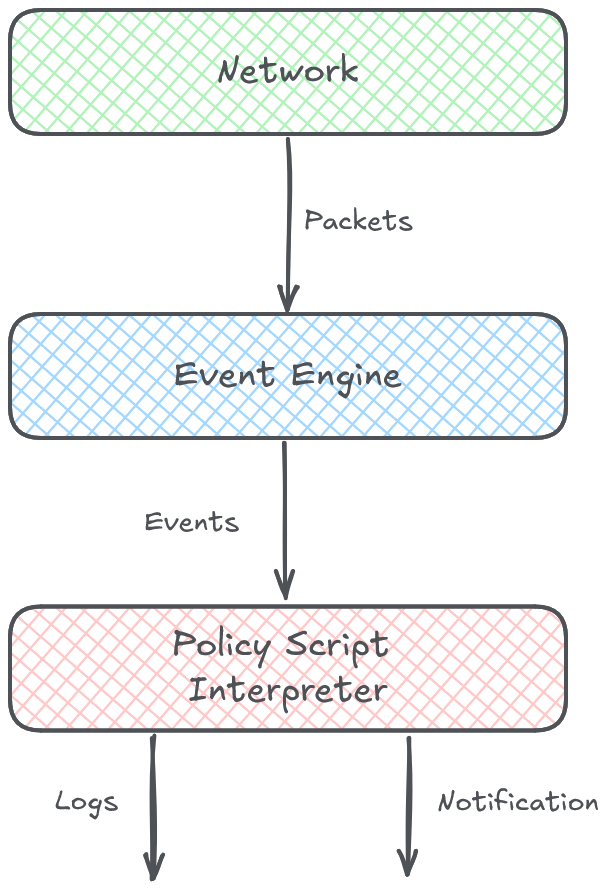
\includegraphics[width=4cm]{./architettura.png}
    \label{architecture}
    \caption{Architecture of ZEEK}
\end{figure}
$\\\\$
The event engine component comprises a number of subcomponents, including in particular the packet processing
pipeline consisting of: input sources, packet analysis, session analysis and file analysis. Input sources 
incest incoming network traffic from network interfaces. Packet analysis process lower-level protocols, 
starting all the way down at the link layer. Session analysis handles application-layer protocols, such as 
HTTP, FTP, and so on. File analysis dissects the content of files transferred over sessions. The event 
engine provides a plugin architecture for adding any of thes from outside of the core ZEEK code base, allowing
to expand ZEEK's capabilities as needed.
\\\\
Semantics related to the events are derived by the second main layer: the \textit{script interpreter}. This 
executes a set of \textit{event handlers} written in ZEEK language. These scripts can express a site's 
security policy, such as what actions to take when the monitor detects different types of activity.
\\\\
More generally scripts can derive any properties and statistics from the traffic. All ZEEK outputs 
comes from scripts included in the distribution. The language can generate real-time alerts and execute 
external programs on demand. One might use this functionality to trigger an active response for attack.
\\\\
With this we had introduced what ZEEK is and briefly how it works.

    %%%%%%% INPUT %%%%%
    \chapter{Input Data}
To make new data similar from some existing ones, we need a dataset of how those data needs to look like.
For this reason we describe di input data, from which we can create new examples.
The inital data needs to be transformed in some way, so it can be given as an input of our GAN.
\\\\
The composition of our dataset is a pcap file. This kind of files contain packet data of a network and are
ofen used to analyze the network characteristics and detect if there're anomalies and intrusions.
Since this kind of data is difficult to manage, even if it's well formatted, a first step is to convert the 
data as a csv dataset.
\\\\
In this way we can easily manage the data before giving them to the network and viewing the final results in a
simpler way.
The pcap file is something like the following:
%image of an extraction of the pcap file
while the output of the conversion of the pcap into the csv is a dataset like:
%image of extraction of the dataset
\section{Data Conversion}
To convert the pcap file into the csv, and viceversa we have created the following script that aims to 
do this kind of transofrmations.
%extract of the script
The foundamental informations are extracted using Scapy \cite{scapy}, a python library used to extract data from packets
saved into a pcap file. The main information that we need are:
\begin{itemize}
    \item the packet number
    \item the protocol used 
    \item the timestamp
    \item the source ip and port
    \item the destination ip and port
    \item the flag if tcp protocol is used
\end{itemize}
from the script we extract those infos from the pcap and store them into the final csv, for each packet into 
the file.
\\\\
Once adjusted the data source, we can continue developing the core of the project: the GAN that generates new
data.

    %%%%%%% DATA GENERATION / GAN%%%%
    \chapter{The GAN}
Developing the GAN poses many question, but the first and most important one is the fact that GANs work better
with continuos input attributes and the data present in our dataset it is not of this kind. For this we have
to apply some tricks so that our data can be given as an input of the Neural Network.
\\\\
Before diving deeper into the implementation of this process it is necessary to discuss what a GAN is.
A GAN o Generative Adversarial Network is a Neural Network used to generate synthetic data by learingn from a
given set of input data. GANs are made of two networks, a generator G and a discriminator D. The generator 
is trained to generate synthetic data from noise. The goal of the discriminator is to distinguish generated 
data from the real word data. The generator is trained iteratively until the generator is able to fool the
discriminator. GANs are really good at generating images, but they have achieved good result also in text
generation or molecule generation.
\\\\
Discriminative models aim to classify objects into predefined classes. In contrast to discriminative models, 
generative ones are used to generate data like the network traffic. Many generative models build on likelihood
maximization for a parametric probability distribution. The generator tries to mimic sample from the data 
distribution, while the discriminator has to differentiate the real and the generated samples.
Both networks are trained iteratively until the discriminator can't distinguish real and generated samples. 
The generator is never updated with real samples. The generator is fed with an input vector of noise 
\textit{z}. So it is trained using only the discriminator's gradient through backpropagation. 
Therefore it is less likely to overfit the generato by memorizing and reproduct real samples.
\begin{figure}[h]
    \centering
    \begin{subfigure}{.45\textwidth}
        \centering
        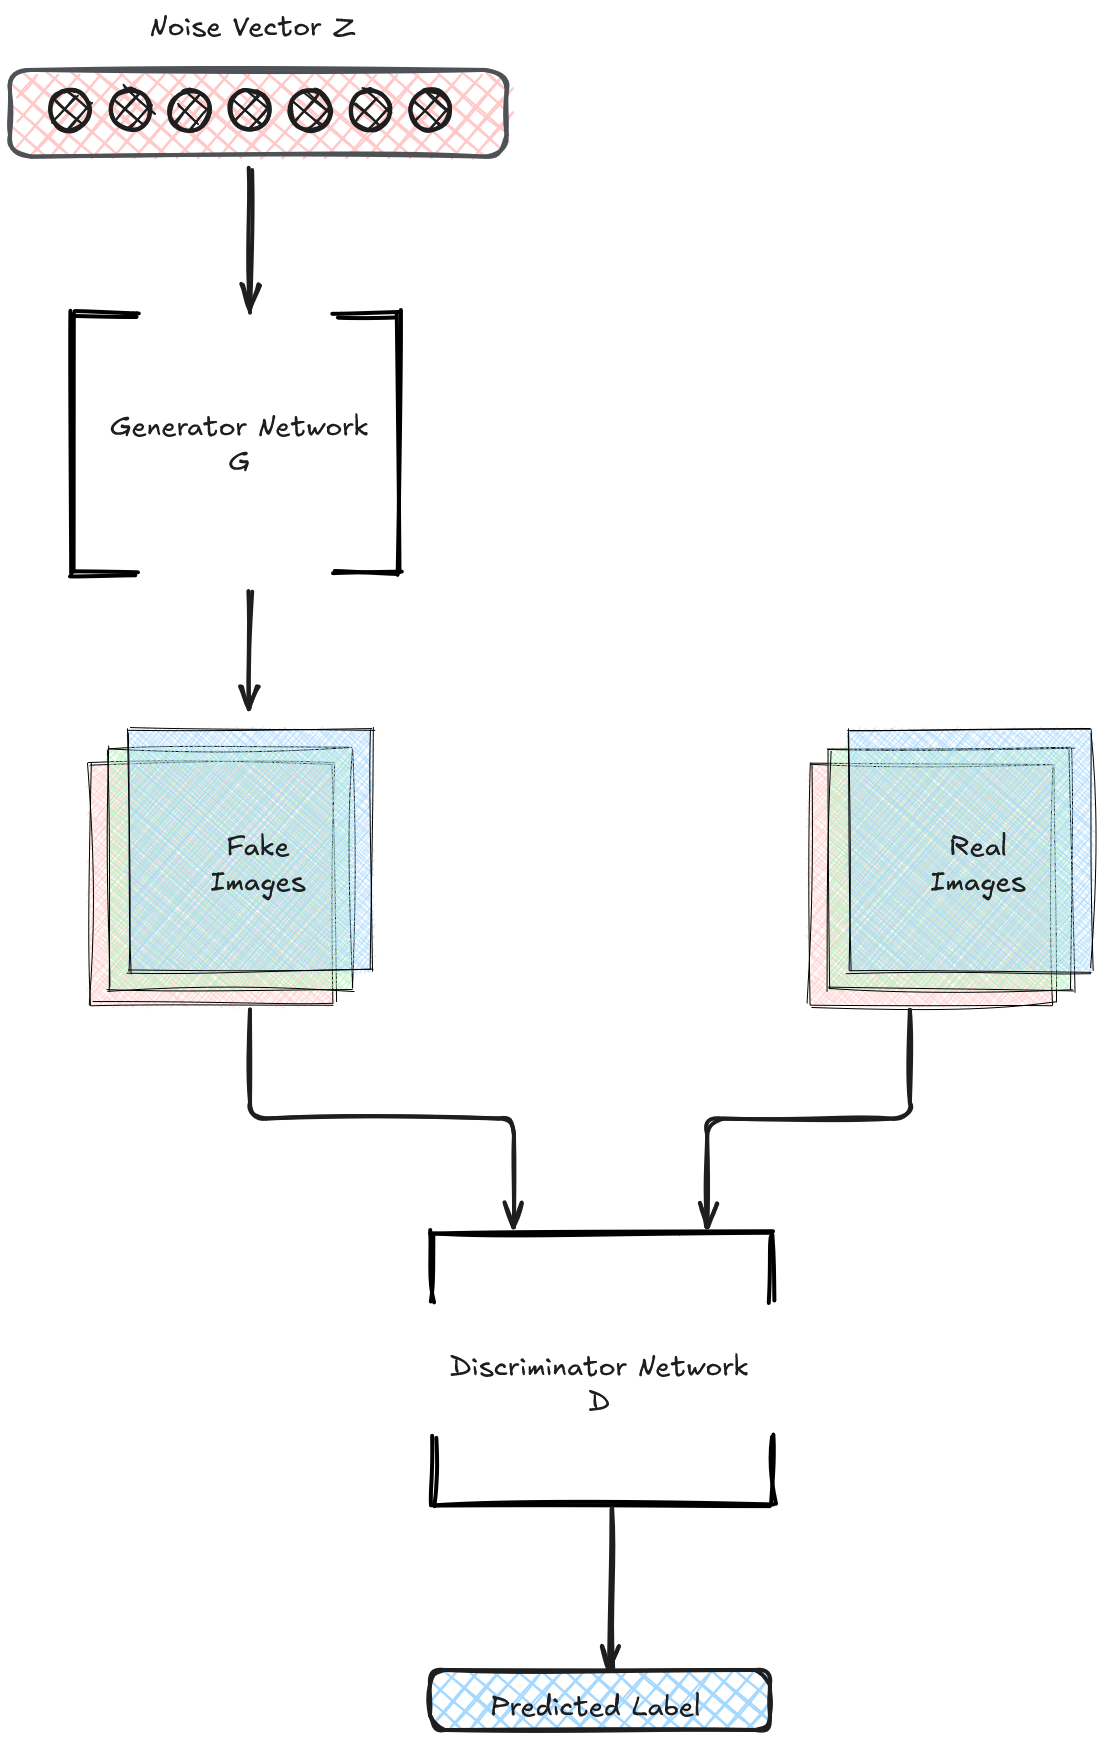
\includegraphics[width=.95\linewidth]{GAN.png}  
        %\caption{}
        \caption{Classic GAN architecture}
    \end{subfigure}
    \begin{subfigure}{.45\textwidth}
        \centering
        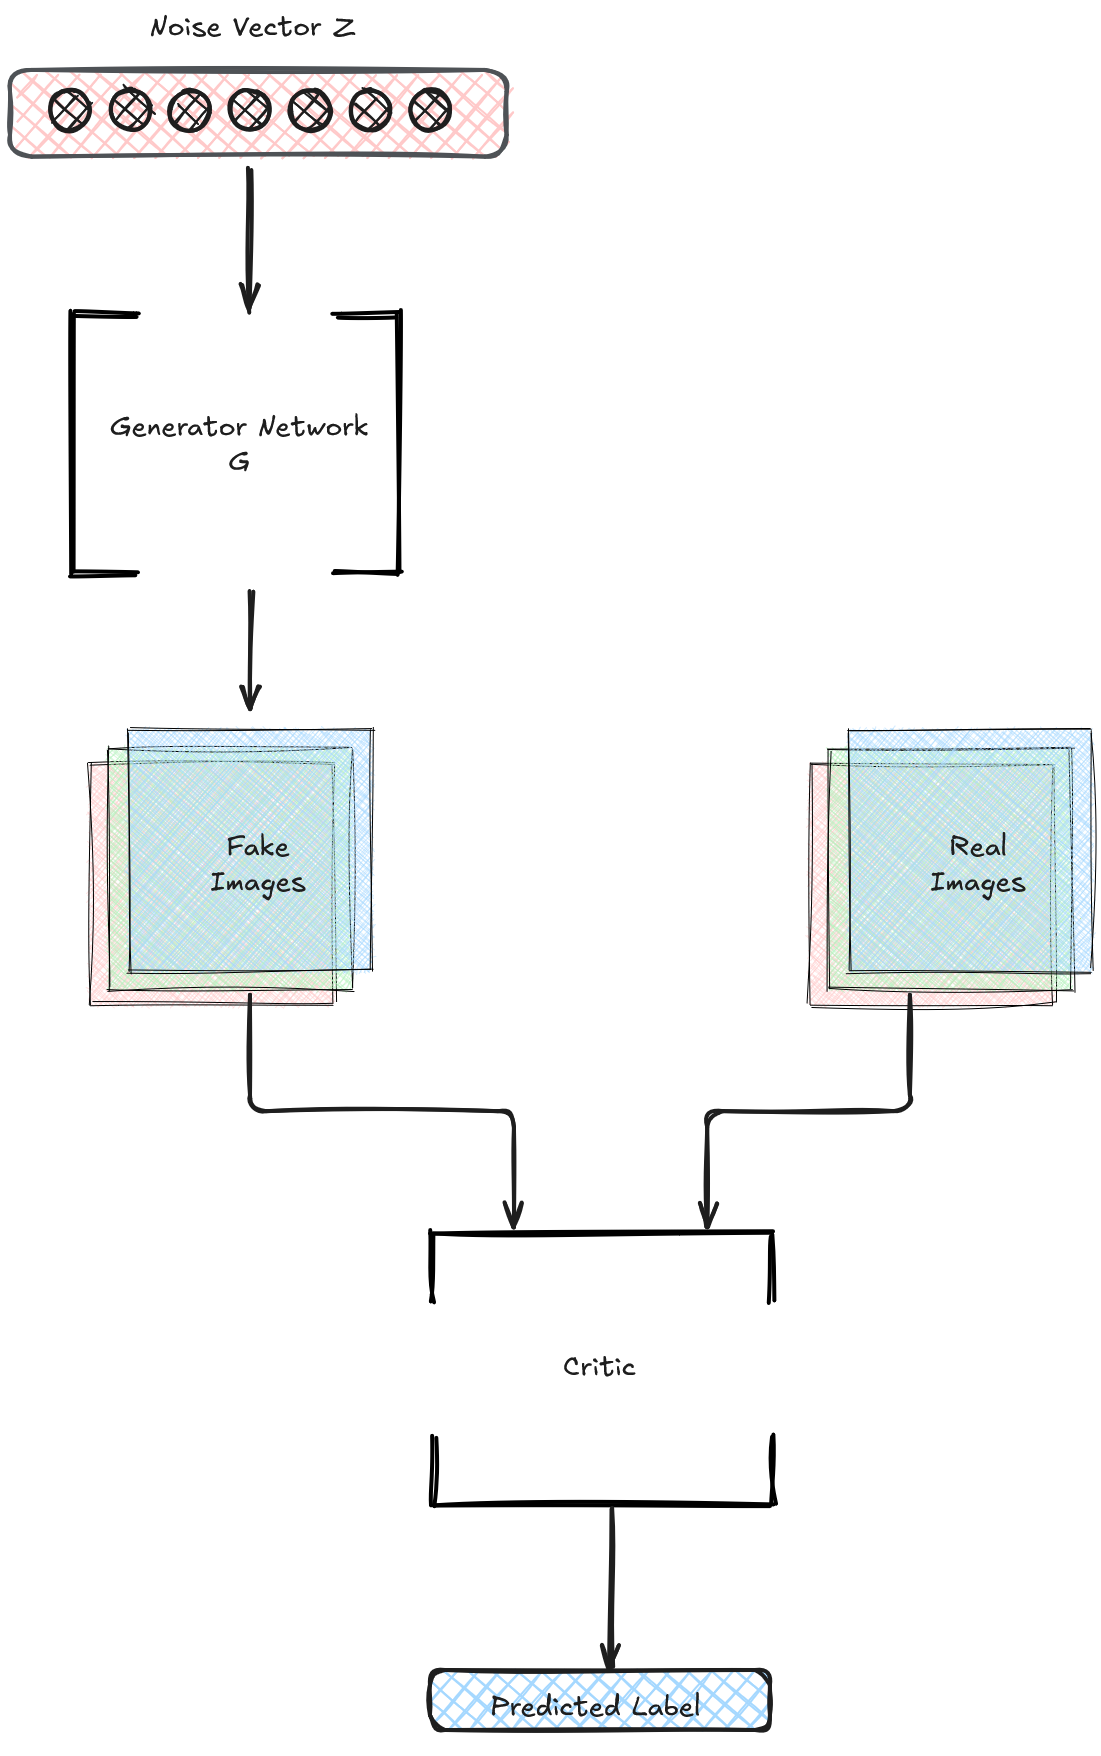
\includegraphics[width=.95\linewidth]{WGAN.png}  
        \caption{Architecture of a WGAN}
    \end{subfigure}
    \label{Architecture differences}
\end{figure}
The vanilla GANs requires the visible units to be differentiable, which is not the case for categorical 
attributes like IPs in the data used. WGANs \cite{wgan} \cite{wgan4n}, are capable of modelling discrete distributions over a continuos
latent space and have other advantages. The main difference is that WGANs uses the Earth Mover (EM) distance 
as a value function replacing the classifying discriminator network with a \textit{critic} network estimating
the distance. To solve the problem of non-convergence in the GANs, it could be useful to apply Two Time-Scale
Update (TTUR) for training GANs with arbitrary functions. For this reason we have choosen to utilize 
WGANs with TTUR.
\section{Preprocessing}
Since the packet capture network traffic that we use as input is made of by both categorical and continuous data,
we need a way to transform the categorical data into continuous ones. There are various methods to do so, one
of them is tho simply treat the attributes like IP and ports as numerical values. The second method could be
to create binary attributes from categorical ones. The last method uses IP2Vec to learna meaningful vector 
rapresentation of the categorical attributes.
\\\\
Since the first two methods are less precise, but are more simple to implement, it has been choosen to 
implement directly the third method even if it is more complex. This due to the fact of attempting to obtain
a better approximation of the input data, and this method works better than the other two.
\section{IP2Vec}
IP2Vec \cite{ip2vec} is a work inspired by Word2Vec and aims to transform IP addresses into a continuous feature space 
$\mathbb{R}^m$ such that standard similarity measure can be applied. To do that we can extract the available
context information from the network traffic. For example the \textit{IP addresses} that appear in similar
contexts will be close to each other in the feature space $\mathbb{R}^m$. This means that similar context 
imply the fact that the devices associated to thes IPs establish similar connections. 
\begin{figure}[h]
    \centering
    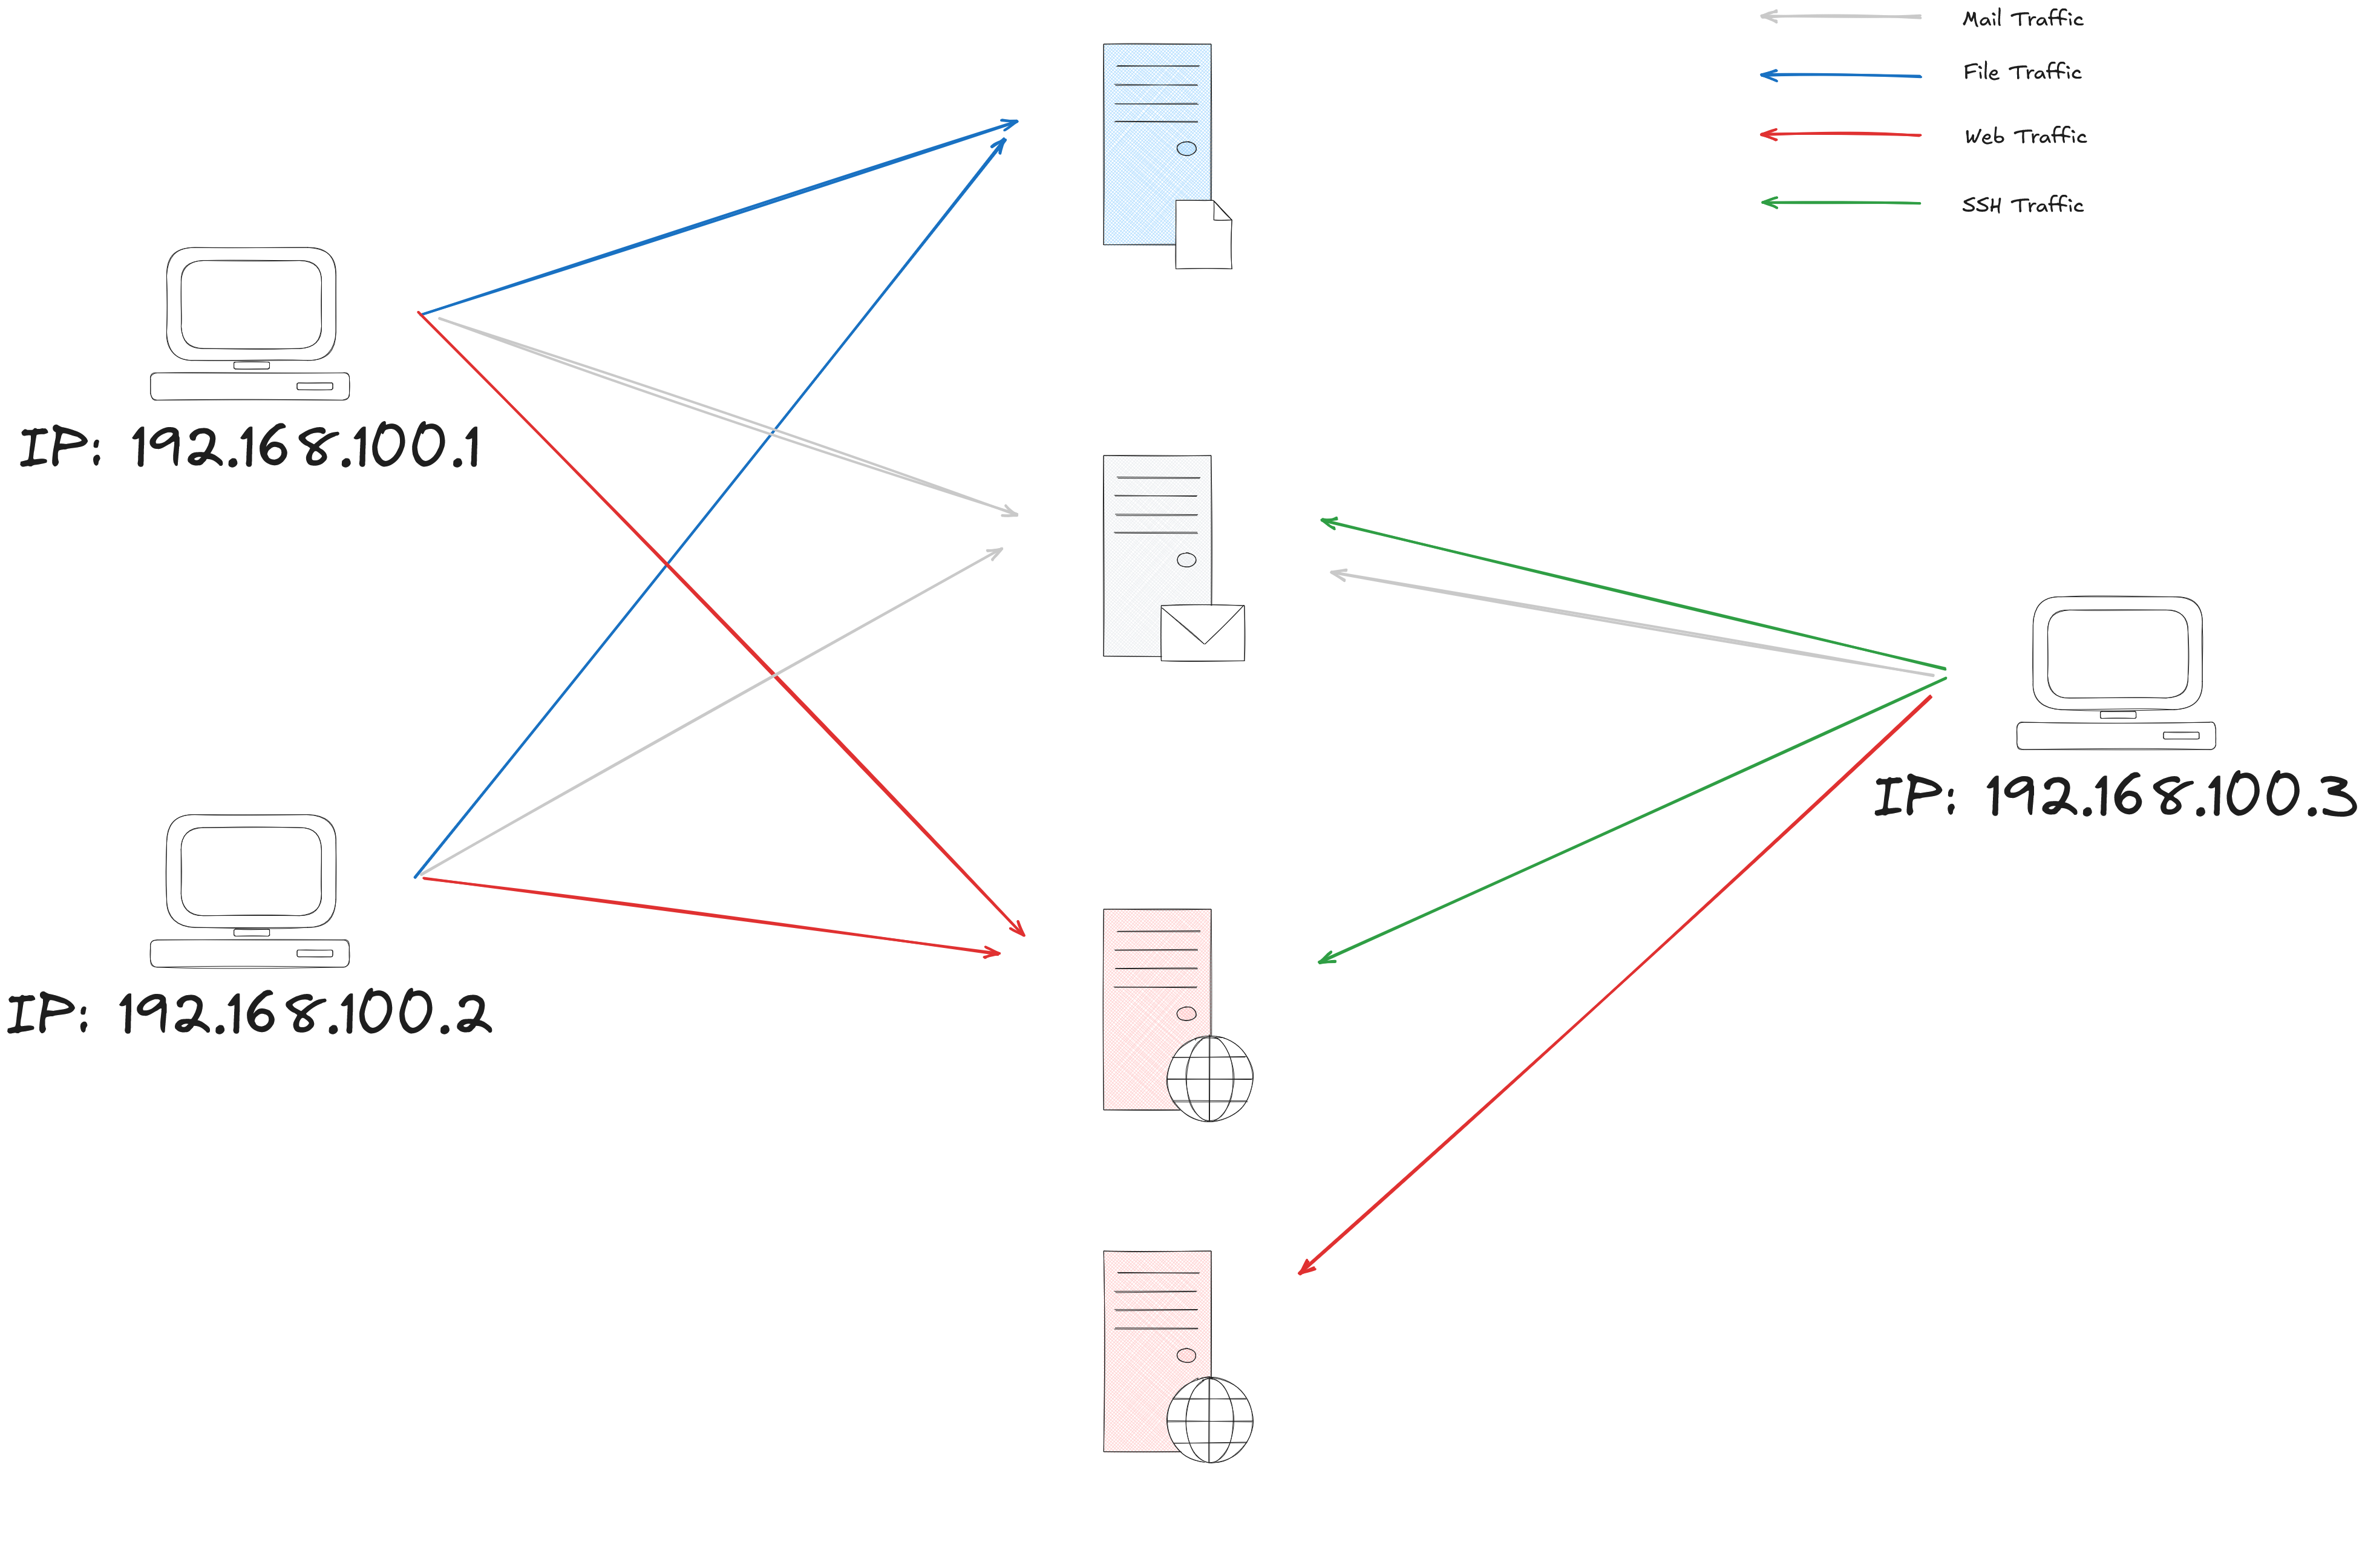
\includegraphics[width=9cm]{IP2Vec_idea.png}
    \label{IP2Vec}
    \caption{Example of connections}
\end{figure}
$\\\\$
In the figure we can see the idea of IP2Vec. The arrows denote network connections from the IPs and the 
different colors indicate different services. From the image we can tderive that the conection made 
by the devices on the left side are more similar that the ones made by, for example, the host $192.168.100.2$
and $192.168.100.3$. This due to the fact that the first couple use the sama kind of connection referred to 
the same targets and services.
\subsection{Model}
IP2Vec is based on a fully connected neural network with a single hidden layer.
\begin{figure}[h]
    \centering
    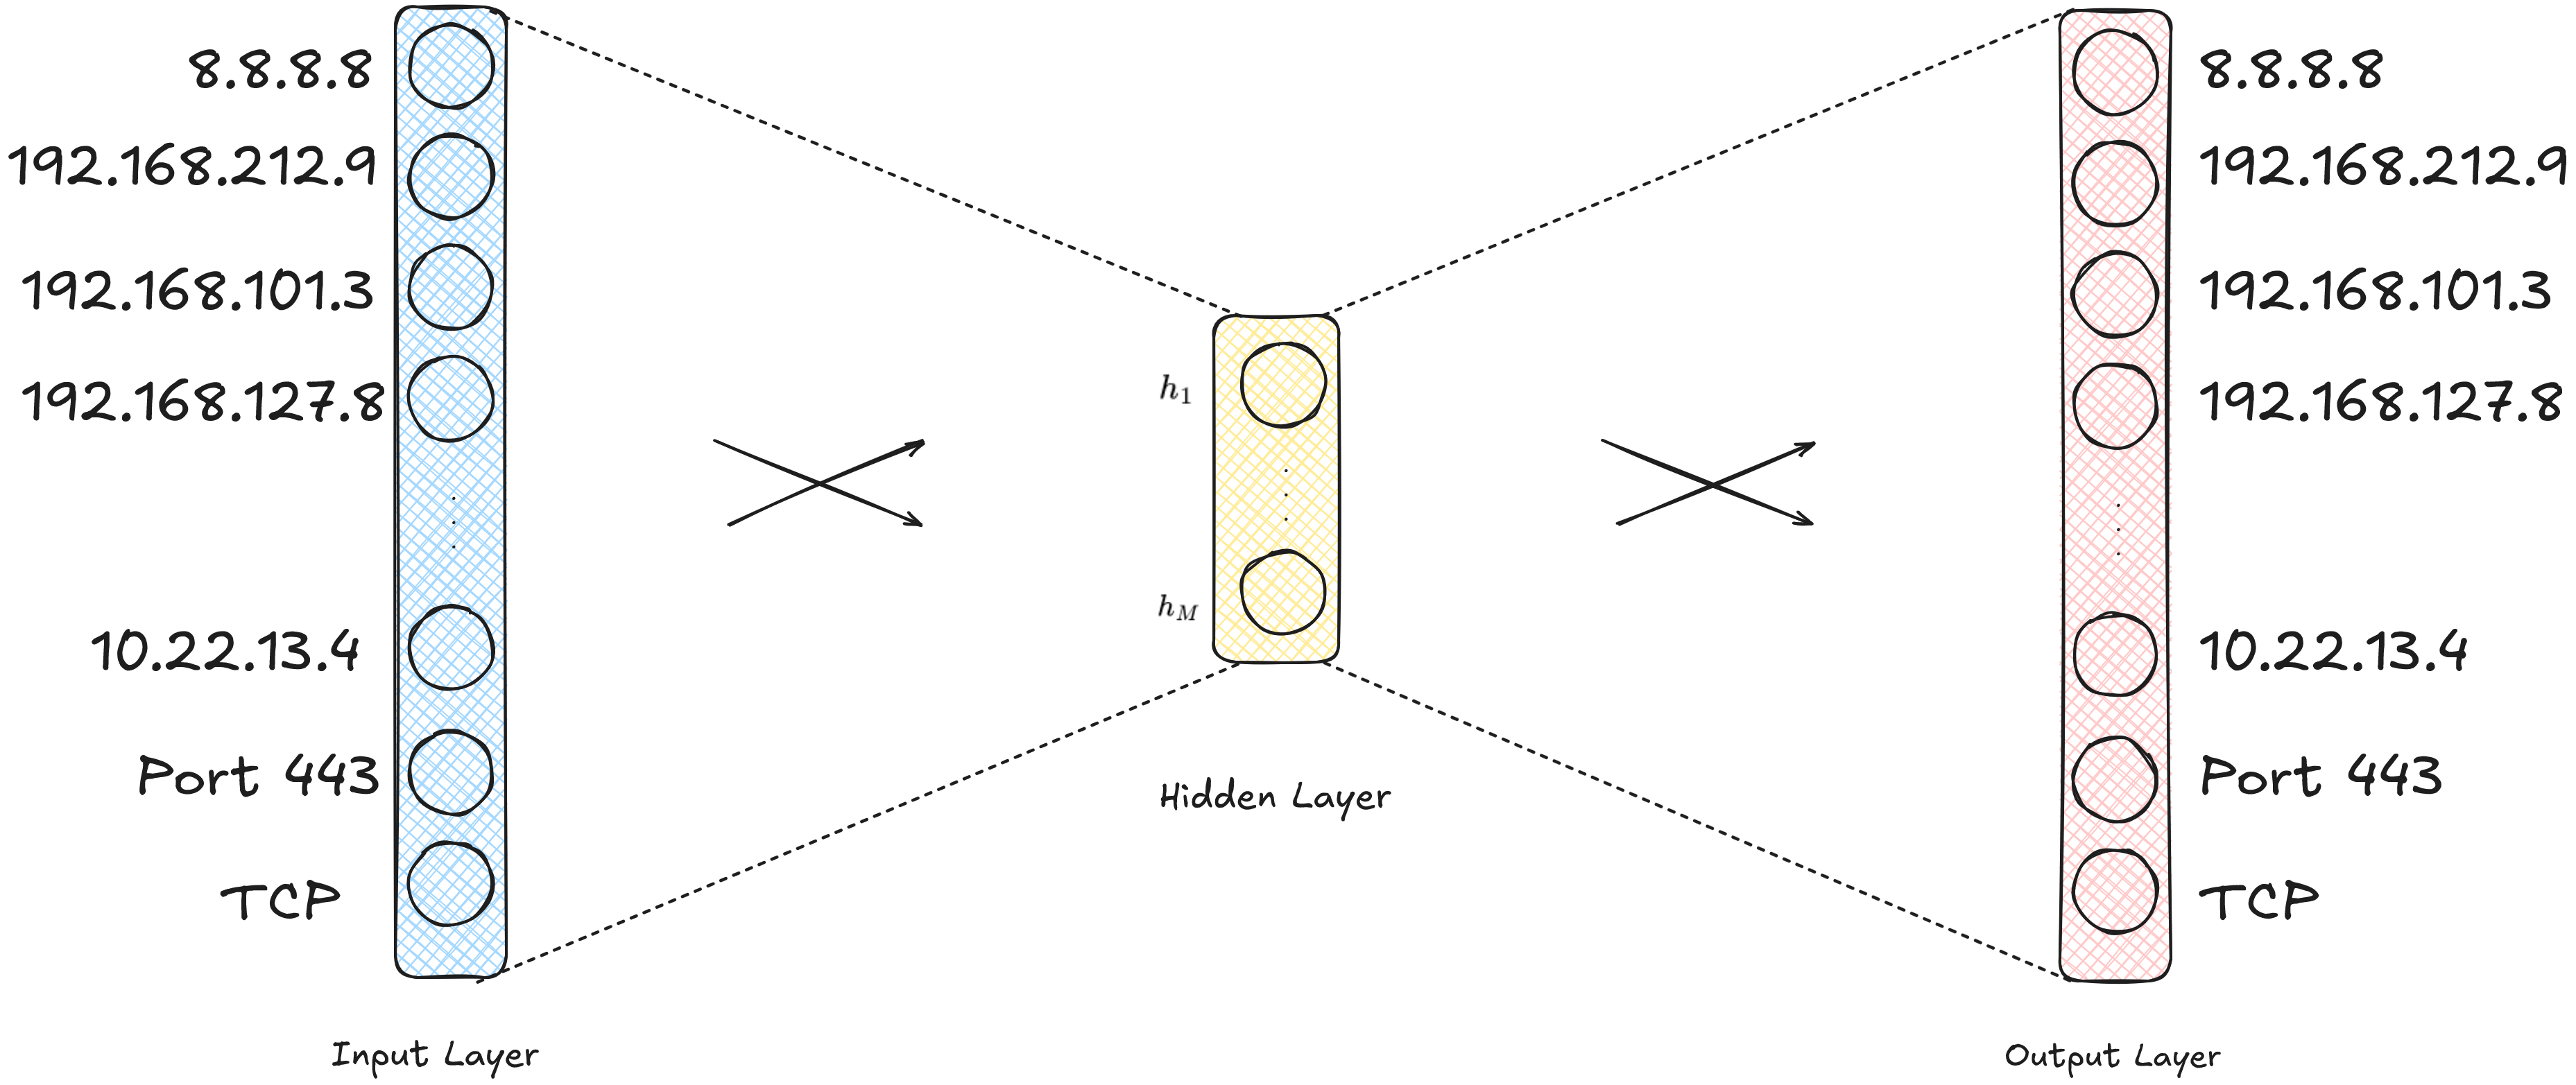
\includegraphics[width=9cm]{IP2Vec.png}
    \label{IP2Vec}
    \caption{Neural Network representation}
\end{figure}
$\\\\$
The features that are extracted from the network traffic consitute the input of the network. The features
consists of the IP addresses, destination ports and trasport protocols and contribute to create the 
vocabulary that contain all of the features that can be seen in the dataset. Since we cannot have categorical
attributes, the vocabulary is represented as a one-hot vector that has the length of the size of the 
vocabulary. 
\\\\
Each neuron in the input and output is then assigned to a specific value of the vocabulary.
The output layer uses a softmax classifier that indicates the probability of each value of the vocabulary 
that it appears in the same context as the input given. The classifier normilizes the output such that the 
sum is 1.
\subsection{Train}
In the training process the neural network is fed with the input value and it tries to predict the probability
of the other values from the vocabulary. For the trining samples the probability of the concrete output value
is 1 and 0 for all the others. The network uses back-prpagation for learning. 
\\\\
With that, we conclude the digression on how the input data is transformed in a way that can be fed to the 
GAN. Since the data generated is then reproduced as an embedding vector it needs also to be converted in a
format similar to the dataset, for that we have used a script that implement that feature


    %%%%%%% DEPLOY %%%%%%%%%%%%%
    %\input{chapter/cap4.tex}
    %%%%%%% END %%%%%%%%%%%%%%%%
    \chapter{Results}

    %%%%%%% BIBLIOGRAPHY %%%%%%%
    \printbibliography[heading=bibintoc]
\end{document}
